%% Energy balancing versus mood lighting: the TKF Dirichlet process
%% Molecular Biology and Evolution -- Methods manuscript, first draft.
%%
%% HAND-MAINTAINED.  Paper 3 of the set; companion to
%%   ../paper1-baumwelch/mbe_paper1.tex  (cited as HolmesLarge2026BW, submitted)
%%   ../paper2-coupled/mbe_paper2.tex    (cited as LargeHolmes2026Coupled, submitted)
%% It must not duplicate either: EM for TKF, the gravestone SCFG, the pair-chain
%% parameterizations, the M-steps and the path ELBO are cited, not restated.
%% The one piece of reused material is the Galton--Watson / lottery-ticket
%% trajectory figure of the retired math-paper (fig:trajectory).
%%
%% Much of the introduction, the two model sections and the discussion are
%% carried over from the retired PSB draft paper2-definetti.tex (git: cfe9496^).
%%
%% Formatting follows the "Manuscript formatting" section of the MBE author
%% guidelines, exactly as papers 1 and 2 do.

\documentclass[11pt]{article}

\usepackage[letterpaper,margin=25mm]{geometry}
\usepackage[utf8]{inputenc}
\usepackage[T1]{fontenc}

%% MBE cites by author and year: "(Cohn et al. 2010)".
\usepackage[round,authoryear]{natbib}
\setcitestyle{aysep={}}

\usepackage{setspace}
\usepackage{amsmath,amssymb,amsfonts,bm}
\usepackage{graphicx}
\usepackage{booktabs}
\usepackage{array}
\usepackage{microtype}
\usepackage{xcolor}
\usepackage{url}
\usepackage[hidelinks]{hyperref}
\usepackage[mathlines]{lineno}
\usepackage{cleveref}   % must be loaded after hyperref

%% lineno does not number displayed equations unless the amsmath environments
%% are wrapped in linenomath.  This is the standard patch.
\newcommand*\patchAmsMathEnvironmentForLineno[1]{%
  \expandafter\let\csname old#1\expandafter\endcsname\csname #1\endcsname
  \expandafter\let\csname oldend#1\expandafter\endcsname\csname end#1\endcsname
  \renewenvironment{#1}%
     {\linenomath\csname old#1\endcsname}%
     {\csname oldend#1\endcsname\endlinenomath}}
\newcommand*\patchBothAmsMathEnvironmentsForLineno[1]{%
  \patchAmsMathEnvironmentForLineno{#1}%
  \patchAmsMathEnvironmentForLineno{#1*}}
\AtBeginDocument{%
  \patchBothAmsMathEnvironmentsForLineno{equation}%
  \patchBothAmsMathEnvironmentsForLineno{align}%
  \patchBothAmsMathEnvironmentsForLineno{gather}%
  \patchBothAmsMathEnvironmentsForLineno{multline}%
}

\crefname{subsection}{section}{sections}
\Crefname{subsection}{Section}{Sections}
\crefname{subsubsection}{section}{sections}
\Crefname{subsubsection}{Section}{Sections}

\newtheorem{defn}{Definition}
\newtheorem{thm}{Theorem}
\newtheorem{prop}{Proposition}
\newtheorem{rem}{Remark}
\crefname{defn}{Definition}{Definitions}
\crefname{thm}{Theorem}{Theorems}
\crefname{prop}{Proposition}{Propositions}
\crefname{rem}{Remark}{Remarks}
\newenvironment{proof}{\par\noindent\textit{Proof.}\ }{\hfill$\square$\par}

\graphicspath{{./figures/}}
\newcommand{\TKF}{\textsc{TKF}}
\newcommand{\TKFDP}{\textsc{TKF--DP}}
\newcommand{\Potts}{\textsc{TKF--Potts}}
\newcommand{\deF}{\textsc{TKF--deFinetti}}
\newcommand{\CTBN}{\textsc{ctbn}}
\newcommand{\CTMC}{\textsc{ctmc}}
\newcommand{\CRP}{\textsc{crp}}
\newcommand{\DCA}{\textsc{dca}}
\newcommand{\MCMC}{\textsc{mcmc}}
\newcommand{\Pfam}{\textsc{Pfam}}
\newcommand{\E}{\mathbb{E}}
\newcommand{\R}{\mathbb{R}}
\newcommand{\Xset}{\mathcal{A}}
\newcommand{\partition}{\mathcal{P}}
\newcommand{\eqm}{\pi}

\begin{document}
\doublespacing
\linenumbers

%% ------------------------------------------------------------ cover page ---
\begin{singlespace}
\thispagestyle{empty}
\begin{center}
{\normalsize Article type: Methods\par}
\vspace{1.5em}
{\Large\bfseries Two substitution processes for a coevolutionary indel model:
energy balancing versus mood lighting at Chinese-restaurant tables\par}
\vspace{1.5em}
{\large Annabel Large$^{1}$ and Ian Holmes$^{1,\ast}$\par}
\vspace{1.2em}
\begin{minipage}{0.85\textwidth}\centering
$^{1}$Department of Bioengineering, University of California, Berkeley,
Berkeley, CA 94720, United States of America\\[0.6em]
$^{\ast}$Corresponding author: Ian Holmes, \texttt{ihh@berkeley.edu}
\end{minipage}
\end{center}
\end{singlespace}

\vspace{2em}

\begin{singlespace}
\noindent\textbf{Abstract}

\noindent We add residue coevolution to the TKF92 indel model without changing
its prior on alignments. In the TKF Dirichlet process (TKF--DP), each residue draws a
key from a Dirichlet process when it is inserted. Residues holding the same
key sit at the same Chinese-restaurant table and evolve under a joint
substitution process. Because keys are drawn independently of the indel
process, the alignment marginal is exactly that of TKF92. As residues join and
leave tables, reversibility requires marginal-consistency: removing a
tablemate must leave the others' joint stationary distribution unchanged.
Exact likelihoods also depend on unobserved residues that join a table and
die within a branch, unless the table's process is lumpable onto its
observed members. We describe two substitution processes. Energy balancing
places a Potts energy on the table and restores marginal-consistency by
Sinkhorn scaling. Mood lighting drives all guests from a shared latent field,
which makes it lumpable and exchangeable by construction, at the cost of
coupling that acts only through shared regime changes. With at most two guests
per table, any reversible pair chain with the right marginals can serve. For alignment we sample the joint posterior over alignments and
pairings with an infinite pair hidden Markov model, and resample table
assignments after realignment along a tempering ladder. On the held-out
Laminin EGF-like family the sampler recovers the disulfide pattern from
sequence alone, placing all 28 Cys--Cys column pairs among the top 50 pair
posteriors. We also report accuracy on the BAliBASE alignment benchmark.

\vspace{1em}
\noindent\textbf{Key words:} coevolution; insertions and deletions; TKF model;
Dirichlet process; Potts model; de Finetti exchangeability; lumpability;
pair hidden Markov model; Markov chain Monte Carlo.
\end{singlespace}

\newpage
% =============================================================
\section{Introduction}
\label{sec:intro}
% =============================================================

Protein sequences evolve, to a first approximation, by insertions and
deletions (indels) and substitutions. The rates of these events are modulated
by selection on the three-dimensional structure, and interacting sites are
frequently observed to coevolve. This selection produces both rate
heterogeneity (hydrophobic cores, for instance, tolerate fewer mutations) and
epistasis (residues in three-dimensional contact evolve in a coordinated way).
An integrated model of protein structure and phylogenetics should therefore
treat indels, substitutions, rate heterogeneity and epistasis as first-order
phenomena.

This paper presents such a framework, combining indels with substitution
epistasis. We set aside locally correlated rate heterogeneity, the kind needed
for phylogenetic models that partition by domain or secondary structure;
models introducing such local partitions have been developed
elsewhere~\citep{Yang1995,ThorneGoldmanJones96,LargeHolmes2026} and are
natural complements to what we describe. Our starting point is the TKF92
model, which layers a finite-state continuous-time Markov chain (\CTMC) for
independent point substitutions on top of a linear birth--death process for
indels~\citep{ThorneEtAl91,ThorneEtAl92}. Two companion papers develop the
pieces we build on. The first gives closed-form expectation-maximization
(EM) for TKF-family indel models and a sampler for the timed indel histories
that lie behind an alignment~\citep{HolmesLarge2026BW}. The second develops
EM and variational inference for coupled two-site and multi-site
substitution chains, organized by the symmetries of reversibility,
exchangeability and lumpability~\citep{LargeHolmes2026Coupled}. Here we put
the two together.

In extending molecular evolutionary models from point to covariant
substitutions, the arc of the literature runs from energy-inspired approaches
toward statistically convenient models. Direct-coupling analysis
(\DCA)~\citep{Marks2011,Morcos2011,ekeberg2013} reads the coevolutionary
signal off a Potts model over amino-acid identities fitted to the column
frequencies of a fixed multiple sequence alignment (MSA). \DCA\ is the modern
end of a line of thermodynamically inspired ideas rooted in the
Miyazawa--Jernigan contact-energy
matrices~\citep{Miyazawa1985,Miyazawa1993}, precursors to Potts couplings,
and in Miyazawa's alignment partition function~\citep{Miyazawa1995}. From
these roots in statistical physics the modeling literature moves toward
Bayesian statistics (Potts models and hidden Markov models), and the two
substitution processes we introduce sit at the two ends of that trajectory.
They are named after Renfrey Potts~\citep{Potts1952} and Bruno de
Finetti~\citep{definetti1937}, and nicknamed \emph{energy balancing} and
\emph{mood lighting}.

We organize the design by a symmetry principle: keep exchangeability and
reversibility wherever possible, so that later models can relax them in
controlled, justified ways. Exchangeability, in the sense of de Finetti, asks
that the coupling be a property of latent, permutation-invariant labels
rather than of named columns. A Potts model's $O(L^2)$ couplings
$J_{ij}(a,b)$ name ordered column pairs, so the model is tied to a fixed
column layout with no generative account of sites appearing or disappearing.
Wilburn and Eddy's hidden Potts model~\citep{wilburneddy2020} is the
foundational instance of coupling named columns within an evolutionary
model, and it serves the profile of a given family well. Our model
generalizes from a supervised set of match-column labels to a large pool of
reusable labels, assigned at random by a stick-breaking process.
Reversibility, in turn, lets an indel process add and remove covarying sites
coherently. It leads to the requirement we call \emph{marginal-consistency}
(\Cref{sec:consistency}).

Both of our models obey this principle by sharing one skeleton, and they
differ only in the substitution process:
\begin{center}
\begin{minipage}{0.85\textwidth}
\emph{The TKF--DP is TKF92 with substitution trajectories relaxed from
independent to exchangeable: coevolutionary partners are seated at the same
Chinese-restaurant table and share a joint substitution process.}
\end{minipage}
\end{center}
The restaurant metaphor for the Ewens partition is standard~\citep{aldous1985,TehJorBea2006};
any caf\'e with large tables works just as well~\citep{AdhikariPitmanCRP}.
\Potts\ carries the coupling as a static pairwise energy and repairs the
damage it does to the single-site marginals. \deF\ carries the coupling
through a shared dynamic field and is exchangeable by construction. Where
\Potts\ follows Potts models, \deF\ can be seen as a generalization of the
CAT Dirichlet-process mixture~\citep{Lartillot2004}. CAT uses a Dirichlet
process to assign the parameters of a time-homogeneous model to sites; the
TKF--DP uses one to assign a time-inhomogeneous model, whose homogeneity is
restored by conditioning on a latent trajectory shared by the table (the
prevailing mood).

The two models trade off differently. Mood lighting is the cleaner
construction, and its likelihood does not depend on the unobserved residues
that pass through a table within a branch. It gets these properties by
giving up the direct dynamics of coevolution, in which a site's substitution
rates respond to its partner's current state, and it loses held-out
likelihood for that reason. When tables hold at most two guests, the
difference matters less, because any suitable two-site chain can then be used
directly. The coupling costs the alignment prior nothing. What it adds to
inference is a posterior over pairings: an alignment now carries a partition
of its aligned columns. We sample that joint posterior with an infinite pair
hidden Markov model (HMM), and resample the partition after each realignment
with a tempering ladder. The framework lets coevolutionary and statistical
alignment approaches work together. Because the substitution likelihood
leaves the alignment prior untouched, the common practice of conditioning on
an alignment and treating gaps as missing data remains legitimate, while
anyone who wants to model covariation and alignment jointly has an explicit
way to do so.

The rest of the paper defines the TKF--DP (\Cref{sec:skeleton}), derives
the two requirements that indels place on the substitution process
(\Cref{sec:consistency}), describes the two substitution processes
(\Cref{sec:potts,sec:definetti}), and develops the sampler
(\Cref{sec:iphmm,sec:ladder}). \Cref{sec:results} reports disulfide recovery
on a held-out family and alignment accuracy on BAliBASE.

% =============================================================
\section{Materials and Methods}
\label{sec:methods}
% =============================================================

\subsection{The TKF Dirichlet process}
\label{sec:skeleton}

Run TKF92 with insertion rate $\lambda$, deletion rate $\mu$ and fragment
extension probability $r$. When a residue $s$ is born it receives three
latent draws, fixed for its lifetime: a \emph{key} $z_s$, a \emph{site class}
$c_s$, and a per-site rate multiplier $\eta_s$. The keys come from a
Dirichlet process. Stick-breaking weights
$w_k=\beta_k\prod_{l<k}(1-\beta_l)$, with
$\beta_k\sim\mathrm{Beta}(1,\alpha_z)$, are drawn once, and every newborn
residue draws $z_s\sim\mathrm{Cat}(w)$ independently of all other residues, of
the indel history and of the substitution history. At any time the living
residues are partitioned into tables by equality of keys, and each table
evolves under its own joint substitution \CTMC.

\begin{defn}[TKF--DP]
\label{defn:tkfdp}
Fix TKF92 parameters $(\lambda,\mu,r)$, a key concentration $\alpha_z>0$, a
set of site-class stationary distributions $\{\eqm^{(c)}\}$ and a family of
table processes: for each finite multiset of site classes $\bm c_C$, a
reversible \CTMC\ on $\Xset^{|C|}$ with stationary distribution $\eqm_C$.
Generate the indel history by TKF92, deal each newborn residue a key, class
and rate as above, and let the residues at each table evolve under the table
process for the table's current membership. When a residue joins a table its
state is drawn from the table's stationary distribution conditioned on the
current states of the other guests; when a residue leaves, its coordinate is
dropped.
\end{defn}

Because the key, class and rate draws are made at birth, independently of
the alignment path and the substitution history, the joint law factorizes as
\begin{equation}
\label{eq:factorisation}
P(\text{alignment},\partition,\{z_s\},\text{subst})
 = P_{\TKF}(\text{alignment})\cdot P(\partition\mid L_A)\cdot
   \prod_s P(z_s\mid\partition)\cdot
   P(\text{subst}\mid\text{alignment},\{z_s\}),
\end{equation}
where $L_A$ is the number of living sites and $\partition$ the induced
partition. Marginalizing the weights, the partition of any $L$ sites is the
Ewens partition with parameter $\alpha_z$, the Chinese restaurant
process~\citep{ewens1972,aldous1985}:
\begin{equation}
\label{eq:crp-prior}
P(\partition\mid\alpha_z,L) =
\frac{\alpha_z^{K}\prod_{b=1}^{K}(n_b-1)!}{\alpha_z(\alpha_z+1)\cdots(\alpha_z+L-1)}
\end{equation}
for a partition into $K$ tables of sizes $n_1,\dots,n_K$. The expected number
of tables is $O(\alpha_z\log L)$; each additional guest at a table costs a
factor of roughly $1/\alpha_z$, so a $k$-clique is suppressed by
$\alpha_z^{-(k-1)}$, and $\alpha_z\to\infty$ recovers independent sites. The
prior is sparse without any penalty on individual couplings. Two further
discrete structures organize the substitution side: a site-class mixture
fixing the background compositions $\eqm^{(c)}$, as in
CAT~\citep{Lartillot2004}, and, in \Potts, a Dirichlet process over coupling
matrices that lets distinct class pairs share a coupling
(\Cref{sec:potts}). Dirichlet processes have previously been used to
partition alignment columns into site classes and sequences into functional
classes~\citep{huelsenbeck2006,huelsenbeck2007,brown2008,nguyen2013,rodrigue2021};
here the partition is over living residues, and it is carried through
insertion and deletion.

\Cref{eq:factorisation} is what lets the TKF--DP keep the TKF92 pair HMM.
Summing out the substitution factor leaves the TKF92 alignment prior at every
value of $\alpha_z$. What \Cref{eq:factorisation} does not say is what the
substitution factor depends on. Tables gain and lose guests along a branch,
so the substitution likelihood of the observed residues can depend on parts
of the indel history that the alignment does not record, and on where the tree
is rooted. The next section takes these two problems in turn.

% -------------------------------------------------------------
\subsection{Tables, indels and augmented histories}
\label{sec:consistency}
% -------------------------------------------------------------

\begin{figure}[p]
\centering
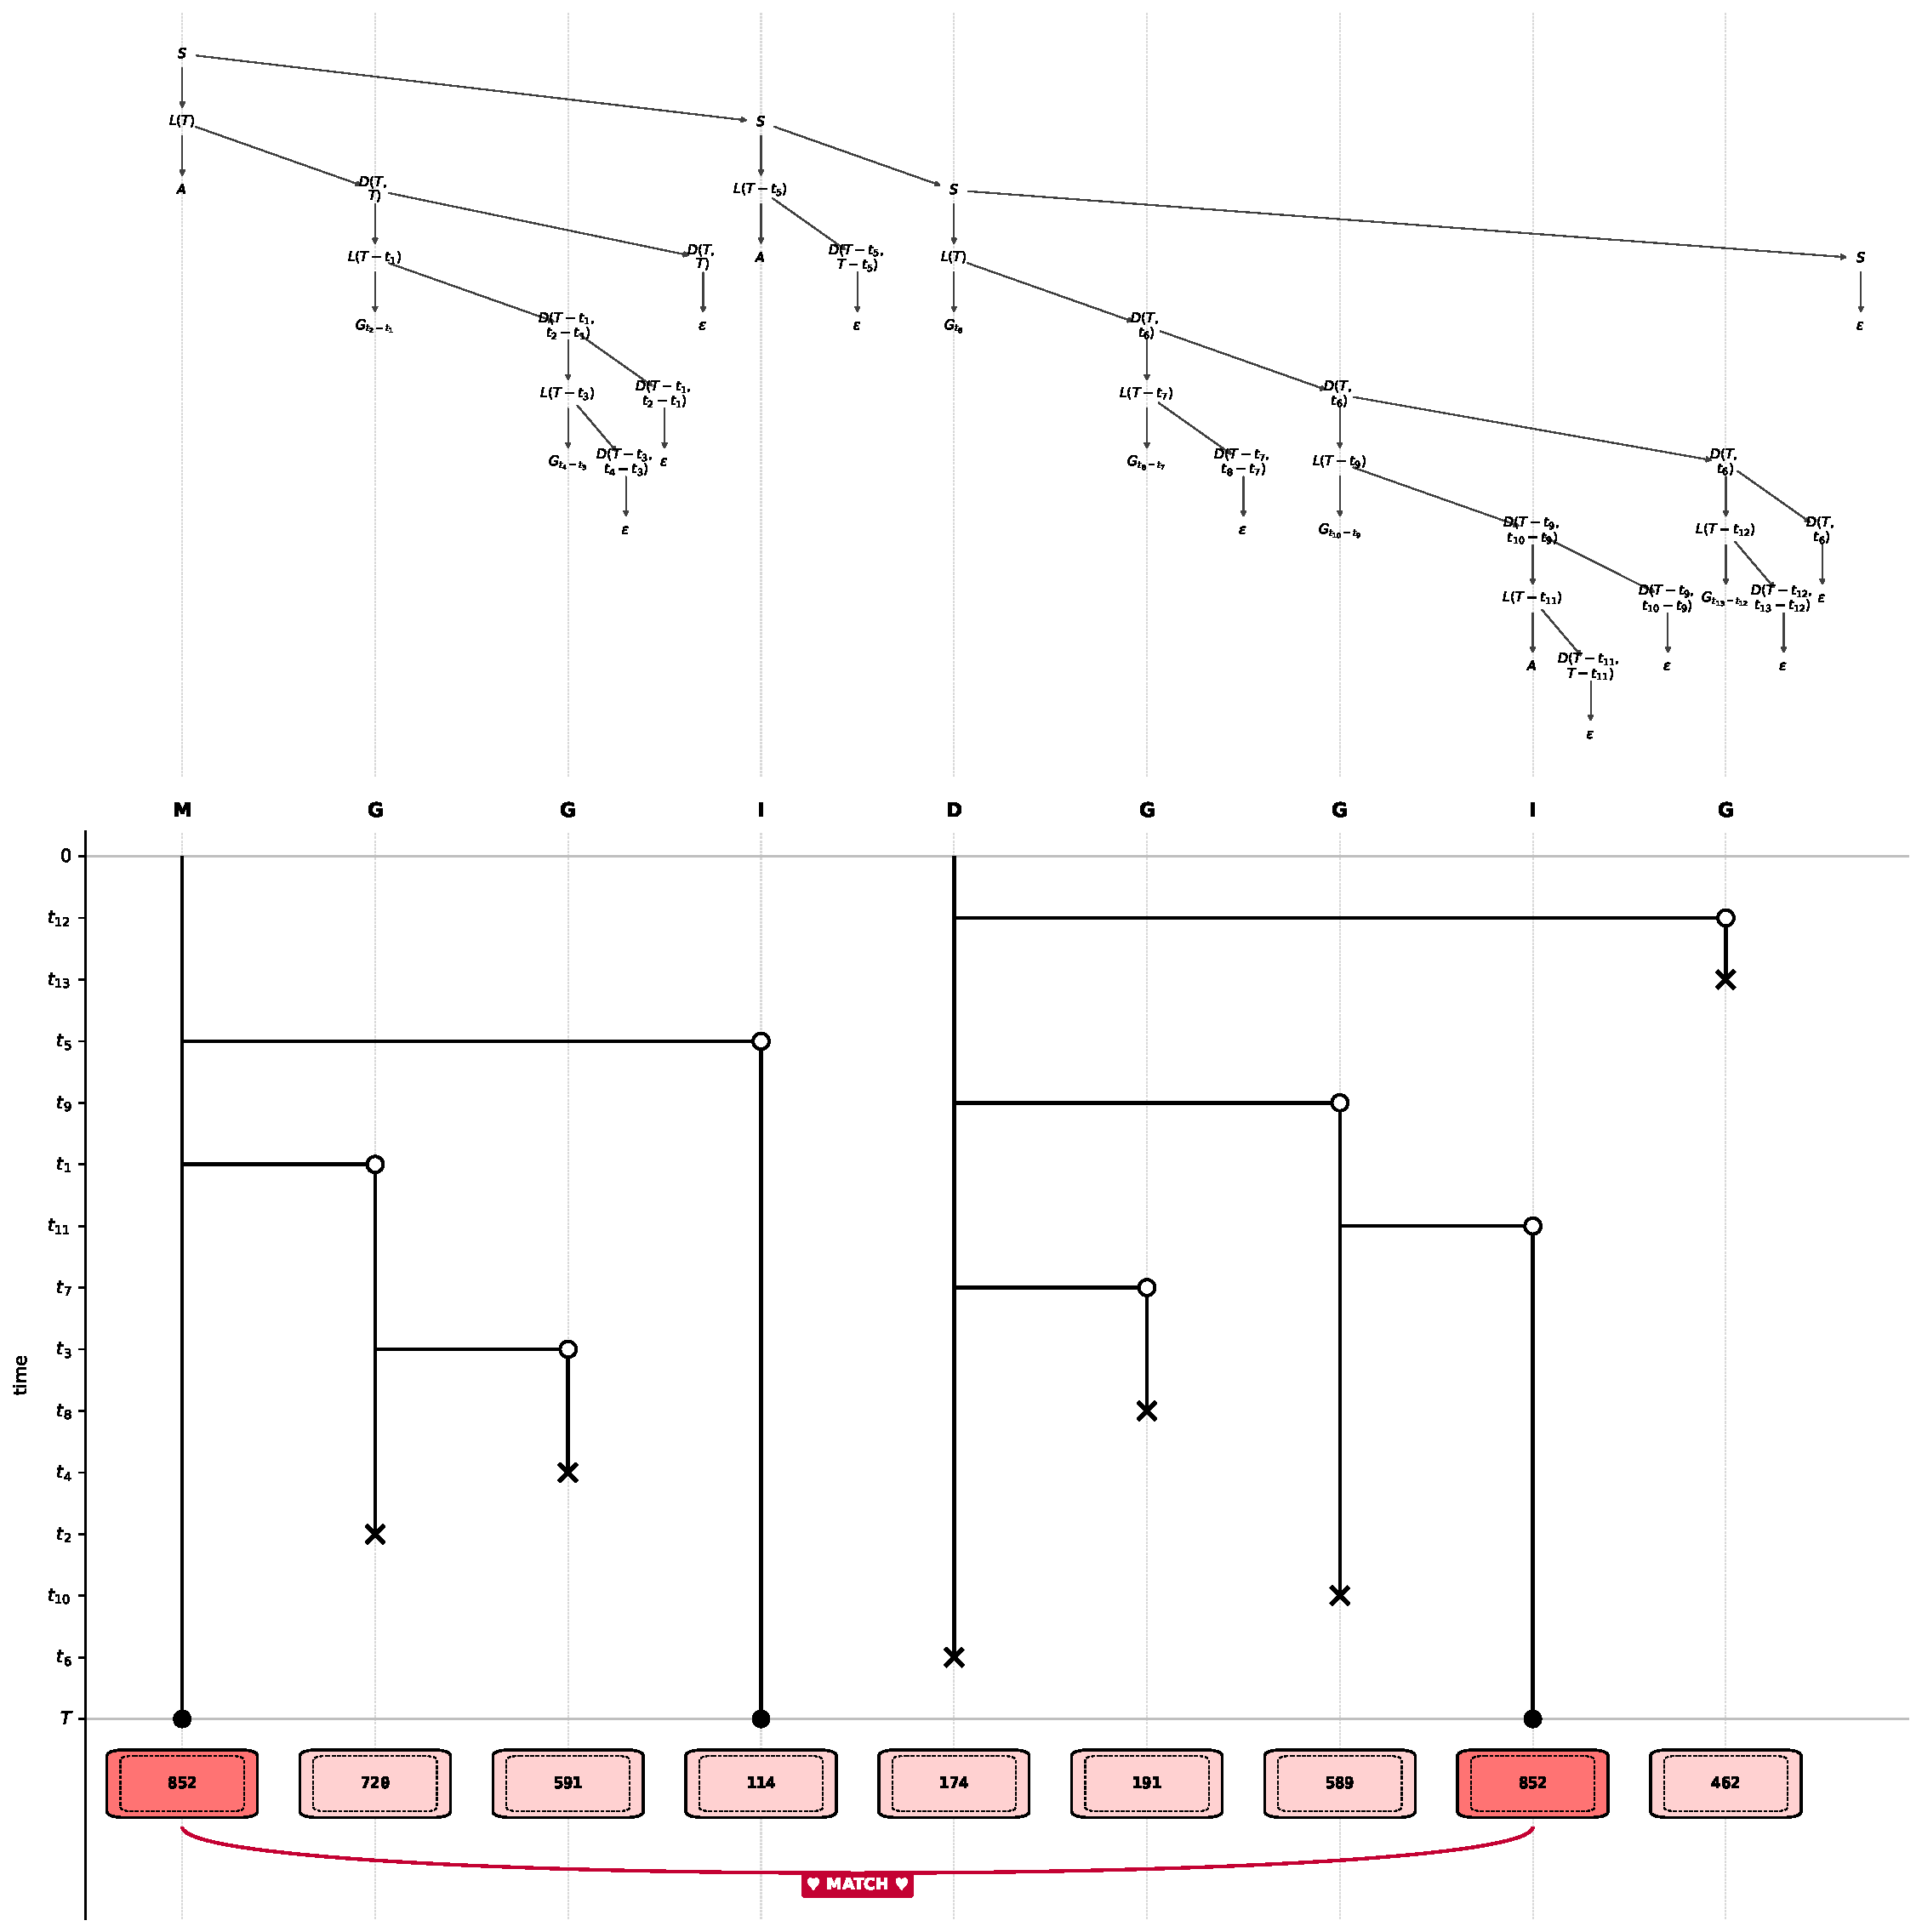
\includegraphics[width=\textwidth,height=0.72\textheight,keepaspectratio]{tkf_trajectory_uber.pdf}
\caption{\textbf{A TKF91 indel trajectory, its gravestone-augmented parse, and
the keys that seat residues at tables.} \textit{Middle:} one realization of
the continuous-time process on a branch of length $T$. Columns are residue
lineages and time runs downward. Open circles mark births, filled circles
survival to $T$, and crosses deaths. The ancestral residue M survives. The
insertion I in column 4 is born at $t_5$ and survives. The ancestral residue
D dies at $t_6$ after spawning three transient lineages (G); the second of
these spawns the surviving insertion I in column 8 at $t_{11}$ before itself
dying at $t_{10}$. \textit{Top:} the parse tree of the same history under the
time-indexed gravestone-augmented grammar of the companion
paper~\citep{HolmesLarge2026BW}, with each nonterminal annotated by its time
arguments. \textit{Bottom:} each lineage draws a key (red lottery ticket)
from the Dirichlet process at birth. Most keys are unique, but the ancestral
residue M and the insertion born at $t_{11}$ both draw key 852 and so sit at
the same table. Before $t_{11}$, M evolves alone; from $t_{11}$ on, its
substitutions are coupled to its new tablemate. Had a transient lineage drawn
852 instead, M would have been coupled for that lineage's lifetime only,
leaving no trace in the alignment.}
\label{fig:trajectory}

{\footnotesize\itshape Alt text: A three-part diagram. The middle panel shows
nine vertical residue lineages over a time axis from 0 to T, with births,
deaths and survivals marked and horizontal arrows for insertion events. The
top panel shows the corresponding grammar parse tree. The bottom row shows
nine red ticket-shaped boxes labeled with three-digit keys; the first and
eighth both read 852 and are joined by a curved line labeled MATCH.}
\end{figure}

\Cref{fig:trajectory} follows one branch of a TKF91 history, which is the
Galton--Watson branching process whose timed histories the companion paper
samples with a gravestone-augmented grammar~\citep{HolmesLarge2026BW}. The
lottery tickets at the bottom are the TKF--DP keys. The ancestral residue M
and the residue inserted at time $t_{11}$ share key 852. The coupling between
them therefore switches on at $t_{11}$, a point in the middle of the branch
that the alignment does not record. Up to $t_{11}$, M substitutes as a
singleton under its class's single-site chain; afterwards it substitutes as
one half of a coupled pair. The substitution likelihood of M's column
depends on when $t_{11}$ fell. Worse, any of the five transient lineages in
the figure could have drawn key 852. It would then have joined M's table,
perturbed M's substitutions for its lifetime, and died without appearing in
either sequence.

Two consequences follow, and they must be kept apart. The first concerns
reversibility. The second concerns whether the unobserved part of the
history can be ignored.

\paragraph{Marginal-consistency is forced by reversibility.} Write the
augmented state of a table as the set $C$ of living guests together with
their residues $x_C\in\Xset^{C}$. Its generator has three parts: substitution
within a fixed $C$, reversible with respect to $\eqm_C$; deletion of a guest
at the residue-independent rate $\mu$; and insertion of a guest at rate
$\lambda$, whose residue is drawn from some insertion kernel
$g_C(y\mid x_C)$.

\begin{thm}[Reversibility criterion]
\label{thm:revcond}
Suppose the within-table \CTMC\ is reversible with respect to $\eqm_C$ and
the candidate stationary distribution of the augmented process factors as
$P(C,x_C)=\omega_{|C|}\,\eqm_C(x_C)$. The augmented process is reversible,
equivalently its phylogenetic likelihood is independent of the root, if and
only if the family $\{\eqm_C\}$ is \emph{marginal-consistent}:
\begin{equation}
\label{eq:consistency}
\sum_{x_s}\eqm_C(x_C)=\eqm_{C\setminus s}(x_{C\setminus s})
\qquad\text{for every table } C \text{ and every } s\in C .
\end{equation}
The insertion kernel is then forced to be the conditional
$g_C(y\mid x_C)=\eqm_{C\cup s}(y\mid x_C)$, and
$\omega_{k+1}/\omega_k=\lambda/\mu$.
\end{thm}

\begin{proof}
Within a fixed $C$, detailed balance holds by assumption. For an insertion
of $s\notin C$ and its reverse deletion, detailed balance reads
$\omega_{|C|}\,\eqm_C(x_C)\,\lambda\,g_C(y\mid x_C)=\omega_{|C|+1}\,\eqm_{C\cup s}(x_C,y)\,\mu$.
Summing over $y$ gives
$\omega_{|C|}\lambda\,\eqm_C(x_C)=\omega_{|C|+1}\mu\sum_y\eqm_{C\cup s}(x_C,y)$.
Both sides are proportional to normalized distributions over $x_C$, so the
constant is one, $\omega_{|C|+1}\mu=\omega_{|C|}\lambda$, and
\Cref{eq:consistency} holds. Substituting back gives the conditional
insertion kernel. Conversely, a marginal-consistent family with that kernel
satisfies every detailed-balance equation.
\end{proof}

A death is residue-independent, so for a birth to be its exact time reversal
the surviving residues must already follow the reduced table's law. When
\Cref{eq:consistency} fails, deleting a partner shifts the survivors'
composition, the likelihood of a column that is gapped in some sequences
depends on where the tree is rooted, and any sampler that moves columns
between tables silently violates detailed balance. The size of the defect is
not academic: on a five-node test tree with one partly gapped pair, the
log-likelihood of the same alignment and partition differed by 1.25 nats
between roots. A raw Potts joint
$\eqm(x_1,x_2)\propto\eqm^{(c_1)}(x_1)\eqm^{(c_2)}(x_2)e^{-H(x_1,x_2)}$
fails \Cref{eq:consistency} at any nonzero $H$, so the condition must be
imposed. Our two models impose it in different ways.

\paragraph{Lumpability removes the dependence on unobserved tablemates.}
Marginal-consistency makes the TKF--DP reversible, but it does not remove
the dependence on $t_{11}$ in \Cref{fig:trajectory}. At stationarity, M's
marginal law is the same before and after its partner arrives, but its
dynamics are not: once coupled, its rates depend on the partner's state. An
exact likelihood must therefore integrate over the times at which tablemates
arrive and leave, including tablemates that never reach a leaf. The
gravestone-augmented grammar of the companion paper~\citep{HolmesLarge2026BW}
supplies exactly that fully augmented history, and it can be sampled.

There is a condition under which none of this is needed. Say that a family of
table processes is \emph{lumpable} if, for every table $C$ and every
$s\in C$, dropping guest $s$'s residue from the table's state (while keeping
any latent state the table carries) leaves a Markov chain, and that chain is
the table process for $C\setminus s$. Lumpability is
the property that the companion paper studies for pair
chains~\citep{LargeHolmes2026Coupled}, extended to tables of any size. When it
holds, a guest's arrival or departure leaves the other guests' law unchanged
along the whole path, not only at stationarity. The discontinuity at
$t_{11}$ disappears, a transient tablemate contributes a factor that sums to
one, and the substitution likelihood of the observed residues depends only on
which observed residues share a table. The alignment and the partition of its
columns then suffice, and no augmented history is needed.

The two properties are nested. Lumpability implies marginal-consistency,
because the stationary distribution of the projected chain is the marginal of
$\eqm_C$, and it must equal $\eqm_{C\setminus s}$. The converse fails.
Marginal-consistency is required of any TKF--DP, since without it the model is
not reversible. Lumpability is optional: it buys indifference to unobserved
tablemates, and, as \Cref{sec:definetti} shows, it has a price.

% -------------------------------------------------------------
\subsection{Energy balancing: \Potts}
\label{sec:potts}
% -------------------------------------------------------------

\Potts\ takes the coupling to be a Potts energy. A Potts model is the
maximum-entropy distribution with prescribed pairwise correlations, and the
direct descendant of the Miyazawa--Jernigan contact energies, so it is the
natural first thing to reach for. Couple two guests of classes $c,c'$ through
a coupling matrix $H_{cc'}\in\R^{20\times20}$. The table's stationary
distribution is the Gibbs form
\begin{equation}
\label{eq:potts-stationary}
\eqm_C(x_C)\;\propto\;\prod_{s\in C}\eqm^{(c_s)}(x_s)\,e^{-g_s(x_s)}
\exp\Big(-\!\!\sum_{\{s,s'\}\subset C}\!\!H_{c_sc_{s'}}(x_s,x_{s'})\Big),
\end{equation}
where the single-site potentials $g_s$ are defined below. The residues evolve
by a single-site chain reversible with respect to \cref{eq:potts-stationary}:
each substitution changes one guest, at a rate modulated by the \emph{current}
states of its tablemates through $H$. This is a continuous-time Bayesian
network (\CTBN)~\citep{nodelman2002} over the table's residues, restricted to
be reversible. It forbids simultaneous substitutions at two guests, so a
compensatory double change passes through a transiently unfavorable
intermediate, and the coupling acts as selection on single-site moves.
Companion work fits pair chains of this kind by EM, together with
alternatives that allow simultaneous changes, and gives a variational lower
bound for tables of more than two guests~\citep{LargeHolmes2026Coupled}.

\paragraph{Balancing the energy by Sinkhorn scaling.} With $g\equiv0$, the
factor $e^{-H}$ in \cref{eq:potts-stationary} distorts the single-site
marginals, and \Cref{eq:consistency} fails. At tables of size two, the
repair is to choose $g_s$ so that each single-site marginal returns to its
class stationary $\eqm^{(c_s)}$. This is matrix scaling of the positive kernel
$\eqm^{(c)}(a)\eqm^{(c')}(b)e^{-H_{cc'}(a,b)}$ to prescribed row and column
sums~\citep{deming1940,sinkhorn1967,cuturi2013}. By Sinkhorn's theorem the
scaled joint exists and is unique, alternating normalization converges
geometrically, and the potentials are unique up to an additive constant at
each site. The scaling leaves every log odds ratio
$\log[\eqm(a,b)\eqm(a',b')/\eqm(a,b')\eqm(a',b)]$ untouched, so $H$ still
carries all the correlation, and only the marginals move. The potentials
cease to be parameters and become a deterministic function of the class
stationaries and $H$.

The repair has a cost. The class of a guest determines its marginal, so a
class's composition cannot depend on who its partner is; site classes carry
composition and $H$ carries correlation. This is one corner of a trade-off:
no table process with at most two guests is reversible, table-independent (a
guest alone at its table follows its class stationary) and able to shift a
class's marginal with its partner, all at once.

\paragraph{Why tables are capped at two guests.} Beyond two guests,
single-site repair no longer suffices. Marginalizing one guest out of a table
whose interaction graph is complete induces a genuine interaction among the
survivors, by graph fill-in. A size-$m$ table carrying a full Potts tensor is
marginal-consistent only if it also carries compensatory potentials of every
order up to $m-1$, fitted Sinkhorn-style so that each lower-order marginal
matches the reduced table. For three guests, the best pairwise-repaired
approximation to the exact three-to-two marginal leaves a residual of about
$10^{-2}$ nats; the residual vanishes only when the fitted order reaches
$m-1$. This tower of compensatory potentials is why \Potts\ caps tables at
two guests. Tables of size two are also the maximal ones that single-site
repair can make reversible.

\paragraph{Sharing couplings across class pairs.} With $K_c$ site classes
there are $K_c(K_c+1)/2$ class pairs, each potentially with its own
$20\times20$ coupling. A further Dirichlet process over coupling matrices
lets class pairs share one, reducing the parameter count from
$O(K_c^2A^2)$ to $O(K_HA^2+K_c^2)$ for $K_H$ distinct couplings and alphabet
size $A$. Evidence then accumulates across families rather than being
refitted for each family, as in \DCA. Sparsity is imposed by which sites
share a table and which class pairs share a coupling, not by a penalty on
$O(L^2)$ free edges.

% -------------------------------------------------------------
\subsection{Mood lighting: \deF}
\label{sec:definetti}
% -------------------------------------------------------------

\deF\ starts from the symmetry principle rather than from a Potts energy. De
Finetti's theorem says that an exchangeable coupling is, necessarily, a family
of processes rendered conditionally independent by a latent directing
variable~\citep{definetti1937,aldous1985}. So rather than have every guest
attend to every other, we hang a single mood light over each table: a latent
field $\theta_C(t)$ that evolves along the tree as its own \CTMC\ and sets
each guest's background composition. For a table with guests of classes
$c_1,\dots,c_m$, the joint state $(\theta,x_1,\dots,x_m)$ evolves by
\begin{align}
\label{eq:field-jump}
(\theta,\bm x)&\to(\theta',\bm x')\ \text{at rate}\
  \rho\,\varrho_{\theta'}\prod_{n=1}^{m}\eqm^{(c_n,\theta')}(x'_n),
  & \theta'&\neq\theta,\\
\label{eq:field-subst}
(\theta,\bm x)&\to(\theta,\bm x\oplus_n y)\ \text{at rate}\
  \eta_n\,S_{x_ny}\,\eqm^{(c_n,\theta)}(y),
  & y&\neq x_n,
\end{align}
where $\varrho$ is the field's stationary distribution, $\rho$ its jump rate,
$S$ the LG08 exchangeabilities~\citep{LG08}, and $\bm x\oplus_n y$ the tuple
$\bm x$ with position $n$ set to $y$. Between field jumps each guest
substitutes independently under a reversible chain whose stationary
distribution $\eqm^{(c_n,\theta)}$ depends on the field. When the light
changes color, every guest is redrawn at once from its new stationary
distribution. Redrawing, rather than carrying the residue across the jump, is
what keeps the compound chain reversible when the field changes the
equilibrium and not merely the rate, which is the distinction between this
construction and covarion models~\citep{tuffleysteel1998}. The field's jump
rule is the F81 form, jumping to $\theta'$ with probability $\varrho_{\theta'}$
regardless of the current state; with $\varrho$ drawn from a Dirichlet
process, this is the parent-independent mutation model whose allelic
partition is again Ewens~\citep{ewens1972,Kingman1975}.

A correlated shift of the guests' compositions at a field jump \emph{is} the
coevolution. Because a single shared cause drives all guests, they are
conditionally independent given the field, and the construction is
exchangeable by construction. It captures a compensatory charge swap
directly: two colors of the light can be the acid--base and base--acid states
of a buried pair. We parameterize the per-class, per-field stationaries
through a shared vocabulary of archetype profiles (LG-C10 or LG-C20
profiles, for example): each pair $(c,\theta)$ maps to one archetype. A class
whose archetype does not change with $\theta$ ignores the field; a class that
switches between a positively and a negatively charged archetype is a
mediator of compensatory change. The site classes, archetypes and field
states are identifiable only up to permutation, as the exchangeable
construction requires.

\paragraph{Mood lighting is lumpable.} No rate in
\cref{eq:field-jump,eq:field-subst} depends on any guest's residue except the
guest being changed. Dropping guest $n$ therefore leaves a Markov chain on
$(\theta,\bm x_{-n})$ with exactly the same rates, that is, the table
process for the reduced table. The light keeps shining whether or not the
table is occupied, so a residue that joins the table at $t_{11}$ draws its
state from $\eqm^{(c,\theta(t_{11}))}$ and leaves the other guests
untouched. Mood lighting is therefore lumpable, and marginal-consistent,
at any table size, with no Sinkhorn step and no tower of compensatory
potentials. A transient tablemate integrates out exactly. Given the field,
the likelihood factorizes over guests, so a table of any size costs one
Felsenstein pass over the small field alphabet.

\paragraph{What mood lighting gives up.} The same property is also a
restriction. Because guests never read one another's residues, a site cannot
respond to its partner's current state; there is no analogue of the rate
modulation that a Potts energy imposes on single-site moves. Correlation
enters only through shared regime changes, and between field jumps the guests
are independent. Mood lighting thus trades the tight dynamics of coevolution
for correlations in the stationary distribution, induced by the field. The
companion paper's comparison of pair chains fitted to substitutions between
residues in structural contact prices this trade-off. Chains lumpable onto
each site share the restriction that neither site's projected dynamics can
depend on its partner. On held-out data they lose $0.015$ nats
($0.022$~bits) per observed pair transition relative to an unrestricted
reversible, exchangeable pair chain, and $0.069$ nats ($0.099$~bits)
relative to the best-fitting chain, a mixture of \CTBN\
components~\citep{LargeHolmes2026Coupled}. They still improve on independent
LG08 sites, by $0.020$ nats, although on data pooled over all contacts the
fitted lumpable chains keep almost none of the stationary correlation either.

\paragraph{Tables of two relax the trade-off.} The restriction matters most
when tables are large, which is where lumpability is most needed. When
tables hold at most two guests, marginal-consistency is a condition on
single-site marginals alone, and any reversible, exchangeable chain on the
400 ordered residue pairs whose single-site marginals equal the class
stationaries can serve as the table process. It can be \Potts's balanced
\CTBN, one of the richer pair chains of the companion
paper~\citep{LargeHolmes2026Coupled}, or a $400\times400$ matrix fitted
directly to contact data. Without lumpability, a pair table's likelihood still
depends in principle on unobserved tablemates. Under the capped Ewens prior
of \Cref{sec:iphmm}, though, a residue already at a table of two cannot
acquire a transient partner, and a singleton does so with probability of
order $\lambda Lt/\alpha_z$ per branch of length $t$, a few percent at the
parameter values we fit. The sampler of \Cref{sec:iphmm} accepts that
approximation, and uses an exact pair likelihood for each coupled pair of
aligned columns.

% -------------------------------------------------------------
\subsection{Inference: the infinite pair HMM}
\label{sec:iphmm}
% -------------------------------------------------------------

Consider two sequences $X$ and $Y$ separated by time $t$. Under the TKF--DP
with tables capped at two guests, the joint posterior over an alignment $A$
and a partition $E$ of its aligned (Match) columns into singletons and pairs
follows from \Cref{eq:factorisation}:
\begin{equation}
\label{eq:iphmm}
P(A,E\mid X,Y)\;\propto\;P_{\TKF}(A,X,Y)\cdot
\frac{\alpha_z^{\,N_M(A)-|E|}}{\prod_{m=1}^{N_M(A)}(\alpha_z+m-1)}\cdot
\prod_{e\in E}\mathcal M(e\mid t),
\end{equation}
where $N_M(A)$ is the number of Match columns of $A$, $E$ is the set of
coupled column pairs, and the middle factor is the Ewens
prior~\eqref{eq:crp-prior} restricted to tables of size at most two. The
first factor is the ordinary TKF92 pair HMM likelihood with independent
single-site emissions, marginalized over site classes. The coupling enters
only through the \emph{boost}
\begin{equation}
\label{eq:boost}
\mathcal M\big((i,j),(k,l)\mid t\big)=
\frac{P_2\big((X_i,X_k)\to(Y_j,Y_l);t\big)}
     {P_1(X_i\to Y_j;t)\,P_1(X_k\to Y_l;t)},
\end{equation}
the ratio of the pair table's joint transition probability for the two
aligned columns to the product of their single-site transition
probabilities, each marginalized over site classes. A boost above one says the
four residues are better explained as a coupled pair. Because the number of
coupled pairs is not capped, this is an infinite pair HMM, in the sense of
the infinite HMM~\citep{Beal2002,TehJordanBealBlei2006}: each alignment
carries an unbounded partition of its Match columns.

We sample from \cref{eq:iphmm} by Markov chain Monte Carlo (\MCMC). Setup
precomputes, once per sequence pair, a partial-Forward tensor giving the
TKF92 pair HMM probability of all alignments passing through Match at any two
anchor cells $(i,j)$ and $(k,l)$, and the boost tensor over all anchor
quadruples. Both take $O(L^4)$ time and memory for sequences of length $L$ and
are reused across all sweeps and chains. A sweep composes three
Metropolis--Hastings moves.
\begin{description}
\item[Segment resampling.] Choose a stretch of the current alignment between
two anchor Match cells and redraw the path between them by stochastic
traceback from the segment's conditional Forward matrix. This proposal is
exact under the TKF92 factor, which therefore cancels from the Hastings
ratio. Coupled pairs with an endpoint in the resampled stretch are dissolved,
and their partners outside become singletons. The acceptance ratio contains
only the prior and boost factors of the dissolved pairs.
\item[Adding a pair.] Choose a singleton Match column and propose a partner
among the other singletons, with probability weighted by boost. The Hastings
ratio combines the prior ratio $1/\alpha_z$ for the new pair, the boost, and
the proposal ratio against the reverse move.
\item[Removing a pair.] Choose an existing pair uniformly and dissolve it;
the ratio is the reciprocal of the matching add move.
\end{description}
The posterior over pairings is multimodal, because a column can be well
explained by several partners, and dissolving a strong pair is rarely
accepted at the trained $\alpha_z$. We therefore run replica exchange
(parallel tempering)~\citep{Geyer1991,HukushimaNemoto1996} over a ladder of
$\alpha_z$ values: chains at larger $\alpha_z$ couple fewer columns and move
freely, and adjacent chains propose to swap states with the usual Metropolis
acceptance. Averaging the Match indicators over post-burn-in samples at the
target $\alpha_z$ gives the posterior probability $Q'_{ij}$ that $X_i$ aligns
to $Y_j$, which replaces the TKF92 match posterior in any downstream
consumer; averaging the pair indicators gives the posterior probability that
two columns share a table.

We checked the sampler against two references. On pairs short enough to
enumerate every alignment and every pairing, the sample means of $Q'_{ij}$
converge to the exact values at the Monte Carlo rate. With $H=0$ every boost
is one, and the sampler recovers the TKF92 match posterior exactly, with the
number of pairs distributed as the capped Ewens prior.

\paragraph{From pairs to multiple alignments.} The posteriors $Q'_{ij}$ from
all pairs of sequences are merged into a multiple alignment by sequence
annealing~\citep{BradleyEtAl2009}, exactly as the TKF92 posteriors are.
Coupled pairs sampled independently in different sequence pairs can also be
projected onto the columns of a family's MSA and pooled. This gives a
composite-likelihood posterior that two MSA columns share a table, which is
how we display coupling across a family in \Cref{sec:results}. The sampler
does not yet share pairings across sequence pairs, and sequence annealing does
not use them.

% -------------------------------------------------------------
\subsection{Resampling table assignments along a tempering ladder}
\label{sec:ladder}
% -------------------------------------------------------------

The pair sampler of \Cref{sec:iphmm} handles pairings crudely when it
realigns: a coupled pair with an endpoint in the resampled stretch is
dissolved, and the move then has to win back any pairing it destroyed through
later add moves. On a tree, where the sampler moves a multiple alignment,
ancestral sequences and topology, the same problem arises for every move
that changes the set of columns. We handle it in our tree-level sampler with a
composite move, \emph{unpair}, \emph{realign}, \emph{repair}, accepted with a
single Hastings ratio against the joint posterior over the history and the
partition. Because a key is drawn at a residue's birth and persists for its
lifetime, the bookkeeping is by column identity. A realignment divides the
columns into those that persist (present, with identical residues, before
and after), those it destroys and those it creates. A coupling survives if
both of its columns persist; a persisting column whose partner is destroyed
becomes a singleton. The realignment is then an ordinary alignment move
scored under the reduced partition, and the repair seats the created columns.

The simplest repair seats the created columns by a draw from the Chinese
restaurant predictive, conditional on the persisting partition. The prior
then cancels from the acceptance ratio, and because the Ewens law is
projective, no factor depending on the number of columns survives. That
repair is exact, but it rarely re-proposes a strong coupling, so a
realignment that destroys a well-supported pair is almost never accepted.
Where a realignment can be bounded by two consecutive paired columns that are
aligned on the branch, it maps singletons to singletons and leaves the
partition unchanged, and no repair is needed. The general case needs a
better repair proposal.

The \emph{annealed repair} replaces the prior draw with a tempered
transition~\citep{Neal1996} along a ladder in the strength of coupling. For
the partition $E_W$ of the created and destroyed columns, with the
persisting couplings held fixed, define
\begin{equation}
\label{eq:ladder-target}
f_\beta(E_W)\;\propto\;P_{\CRP}(E_W\mid E_{\mathrm{red}},\alpha_z)\,
\exp\Big(\beta\sum_{\{i,j\}\in E_W}\Delta(i,j)\Big),
\end{equation}
where $\Delta(i,j)$ is the \emph{coupling excess}: the log-likelihood of
columns $i$ and $j$ as a pair on the tree, minus their log-likelihoods as
two singletons. On a single branch it is the log of the boost
\eqref{eq:boost}. At $\beta=1$, $f_\beta$ is the conditional posterior of the
partition; at $\beta=0$ it is the bare prior. Neither the alignment
likelihood nor the prior is tempered. With a ladder
$1=\beta_0>\beta_1>\dots>\beta_n=0$ (we space it linearly), the move proceeds
as follows.
\begin{enumerate}
\item \textbf{Melt.} Under the old alignment, starting from the current
partition $x_0$, for $k=1,\dots,n$ apply one partition kernel that leaves
$f_{\beta_k}$ invariant, reseating a destroyed column, to obtain $x_k$.
\item \textbf{Realign at the apex.} At $\beta=0$ the destroyed columns carry
no coupling, so the realignment is proposed and scored as an uncoupled
move, and the created columns are seated from the conditional
prior. If a draw lands at a full table of two, the move is rejected.
\item \textbf{Freeze.} Under the new alignment, for $k=n,\dots,1$ apply the
kernel for $f_{\beta_{k-1}}$, reseating a created column, to obtain the
states $y_k$ and finally the proposed partition.
\item \textbf{Accept once.} Accept the whole excursion with the composite
Hastings ratio, in which the coupling terms are replaced by
\begin{equation}
\label{eq:ladder-R}
R=\prod_{k=1}^{n}\frac{f_{\beta_k}(x_{k-1})}{f_{\beta_{k-1}}(x_{k-1})}
\;\prod_{k=1}^{n}\frac{f_{\beta_{k-1}}(y_k)}{f_{\beta_k}(y_k)},
\end{equation}
where each $f$ is evaluated under the alignment current at that stage.
\end{enumerate}
The per-rung kernel is a single-site Gibbs reseat: a column either sits
alone, with weight proportional to $\alpha_z$, or joins an open singleton $j$,
with weight $e^{\beta\Delta(i,j)}$. Only open singletons are candidates, so
the cap of two guests is never violated in the middle of a pass.

The kernels' transition densities cancel in $R$, because each is run forward
while melting and as its reverse while freezing, and the unknown normalizers
of the $f_{\beta_k}$ telescope between the two passes. No importance weight is
stored, and nothing is carried between moves. The construction is exact for
any number of rungs: at $n=0$ it is the prior-draw repair, and more rungs
trade computation for acceptance, not for bias. One application of the kernel
per rung suffices, since no rung needs to be equilibrated. The ladder stacks
on the replica-exchange ladder: a chain run at an elevated coupling
temperature $T$ anneals only from $\beta=1/T$ to $0$. Two ordering details
matter for exactness. The coupling ratio must be read before the kernel is
applied while melting and after it while freezing, and $R$ replaces the
closed-form coupling term of the prior-draw repair rather than adding to it.
We checked the implementation against an exactly enumerated posterior on a
small tree. With one rung and the Potts coupling on, the total variation
distance between sampled and exact distributions was $0.012$ over eight
chains of $360{,}000$ moves, at the Monte Carlo floor of the rung-free move
($0.014$); toy chains with up to five rungs, including moves that change the
number of columns, agree with their exact targets. The ladder is exact, but
we have not yet measured how much it raises the acceptance rate.

% -------------------------------------------------------------
\subsection{Training}
\label{sec:training}
% -------------------------------------------------------------

We fitted two \Potts\ models to \Pfam\ families~\citep{Pfam2021}
by stochastic variational EM, alternating an E-step for the amino-acid
substitution statistics~\citep{LargeHolmes2026Coupled} with Gibbs moves on the
key partition, the site classes and the assignment of class pairs to
coupling matrices. The four-class model ($K_c=4$) was fitted to $1{,}000$
families after an EM warm-up and has $K_H=10$ coupling matrices. The
eight-class model ($K_c=8$) was fitted to $8{,}000$ families and has a single
coupling matrix, since larger numbers of coupling matrices overfit on held-out
data. Both use LG08 exchangeabilities, $\alpha_z=100$, and TKF92 indel
parameters fitted separately by the closed-form EM of the companion
paper~\citep{HolmesLarge2026BW}; for the four-class model these are
$\lambda=0.0458$, $\mu=0.0468$ and $r=0.683$. For the eight-class model,
the largest joint-emission log odds in the fitted coupling are biochemically
sensible: disulfide C--C ($+3.66$ nats), the aromatic stacks W--W ($+3.63$),
Y--Y ($+2.69$) and F--Y ($+1.90$), His--Cys metal coordination ($+1.27$), and the
charge-complementary pairs E--K ($+1.09$) and E--R ($+0.89$).

Both models use the bare Potts joint distribution ($g\equiv0$), restrict pairs
to Match columns, and count only Match columns in the Ewens prior; every result
reported below was computed under that convention. The Sinkhorn balancing of
\Cref{sec:potts} restores marginal-consistency and is implemented in the
sampler, where it is now the default; the fits reported here predate it.
%% PROVENANCE: released checkpoints K4-emwarm-top1000-2026-05-09 and
%% K8-KH1-top8000-2026-05-22 (results/exp2_v2_K8_KH1_top8000_2026-05-22/
%% _best_chkpt/).  src/tkfdp/mcmc_infinite_phmm.py has defaulted to
%% reversible=True (A1, balanced) since 2026-06-27; both checkpoints predate
%% it and were evaluated in legacy (--pre-sinkhorn) mode.  A partial A1
%% K8 retrain exists at results/exp2_v2_K8_KH1_top8000_A1_2026-06-28/
%% (stopped at outer 49/300, best val_LL -49680.02 @ iter 40); it is not
%% used for any number in this paper.  Rerun plan:
%% docs/balibase_187pair_rerun_plan.md.
%% K8 coupling log-odds are from paper2-definetti (PSB), figure
%% k8_coupling_score.pdf.

% =============================================================
\section{Results}
\label{sec:results}
% =============================================================

\subsection{Disulfide recovery on a held-out family}
\label{sec:pf00053}

The Laminin EGF-like domain (\Pfam\ \texttt{PF00053}) is small, cysteine-rich
and indel-punctuated: eight conserved cysteines form four disulfide bonds,
and the loops between them vary in length. The family was held out from
training. We first ran the sampler, with the eight-class model, on a single
sequence pair: two EGF-like
repeats of human laminin subunit $\alpha$-1 (LAMA1; UniProt \texttt{P25391},
residues 1452--1506 and 1090--1147). The two repeats have $55$ and $58$
residues, share only $21\%$ identity and are separated by an estimated
divergence of $t=2.15$, which is diverged enough that the TKF92
alignment posterior is no longer close to deterministic
(\Cref{fig:lama1}c). The joint sampler concentrates pairing mass on Cys--Cys
cells, well above both the background and the samplers run on each sequence
alone (\Cref{fig:lama1}a,b,d,e). In the same analysis with the four-class
model of \Cref{sec:training}, the Cys--Cys enrichment over the background was
$17$-fold within the first sequence and $12$-fold within the second, against
$5$-fold for the single-sequence samplers.
%% PROVENANCE: the quoted enrichments are the four-class run of 2026-05-15,
%% whose cache is committed at
%% math-paper/figures/holmes_tile_PF00053_lama1_test_cache.json
%% (exactly 17.0x / 11.9x / 5.1x / 5.1x).  \Cref{fig:lama1} is drawn from the
%% eight-class run (commit 00c4025), whose cache was not committed; hence the
%% enrichment ratios are quoted for the four-class model and attributed as
%% such in the text.  See docs/balibase_187pair_rerun_plan.md (step 5).
The coupling
also sharpens the alignment posterior around the conserved cysteines
(\Cref{fig:lama1}f).

\begin{figure}[t]
\centering
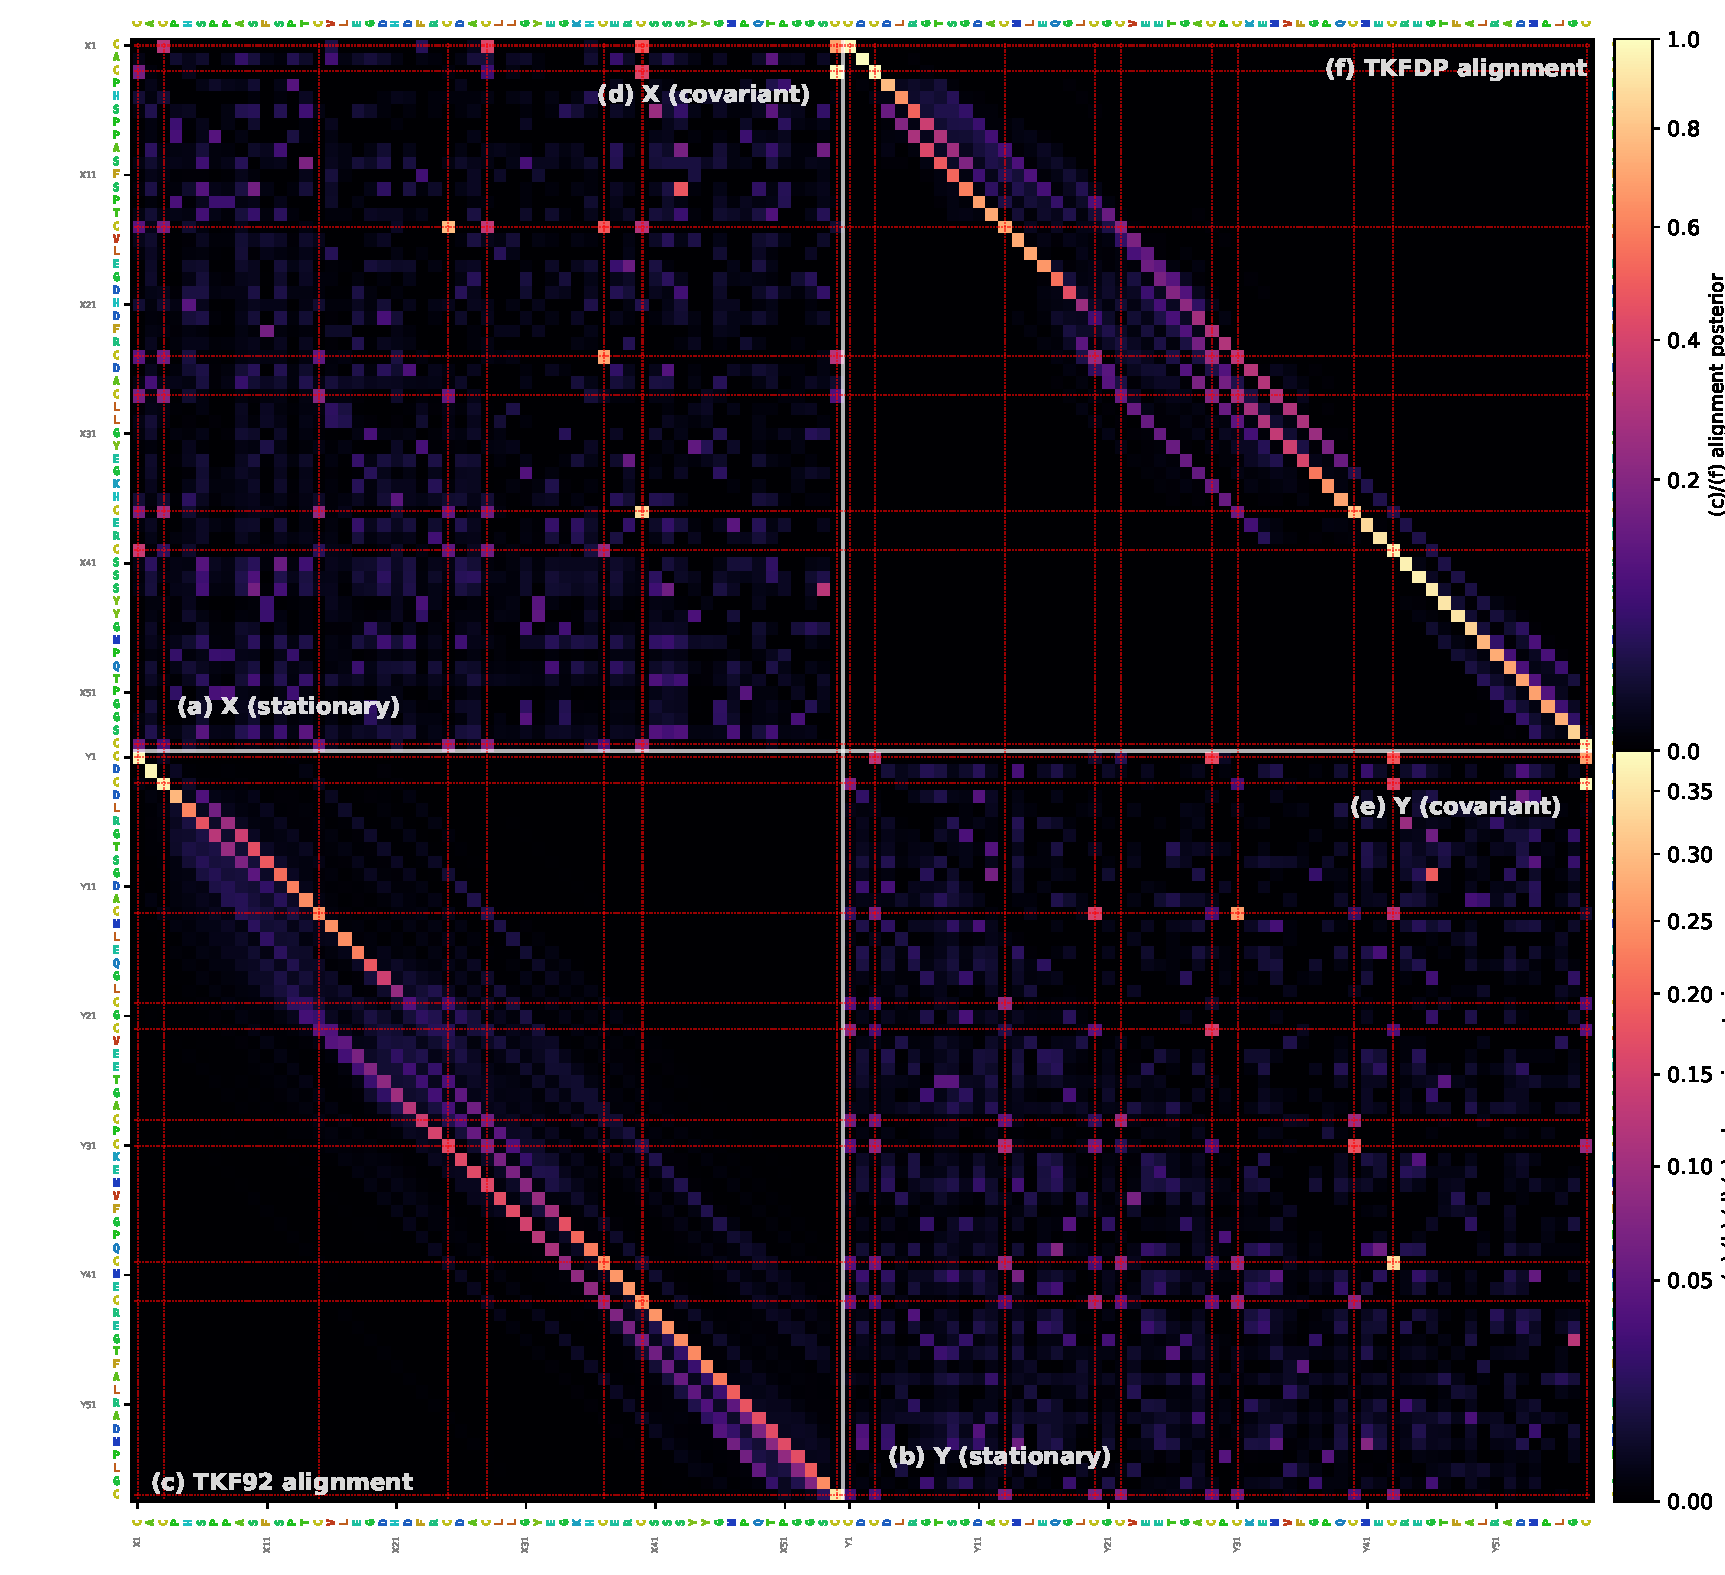
\includegraphics[width=\textwidth]{holmes_tile_PF00053_lama1_test_K8.pdf}
\caption{\textbf{Pairings and alignment for two held-out LAMA1 EGF-like
repeats (\texttt{PF00053}).} Rows and columns are residues of the two
sequences X and Y. \textit{Off-diagonal blocks (c, f):} match posteriors
under TKF92 (c) and under the TKF--DP infinite pair HMM (f). \textit{Diagonal
blocks:} posterior probability that two residues of the same sequence share a
table, from a sampler run on that sequence alone (a, b; stationary pair
distribution only) and from the joint sampler over both sequences (d, e;
coupled dynamics along the branch). Cysteines are marked by red guide lines.
The joint sampler concentrates pairing mass on Cys--Cys cells.}
\label{fig:lama1}

{\footnotesize\itshape Alt text: A square heat map divided into four
blocks by the two sequences. The upper-right and lower-left blocks show
bright near-diagonal alignment posteriors. The upper-left and lower-right
blocks show mostly dark pairing posteriors with bright cells at pairs of
cysteines.}
\end{figure}

Pooling across the family sharpens the signal (\Cref{fig:pf00053}). We ran the
sampler, with the eight-class model, on eight sequence pairs from the
$72$-sequence family alignment,
projected each sampled pairing onto MSA columns, and averaged. The eight
canonical cysteine columns give $28$ candidate Cys--Cys column pairs, and all
$28$ fall within the top $50$ column-pair posteriors (in fact within the
top $41$). The mean Cys--Cys
posterior is $0.087$, against $0.004$ for other column pairs, about $22$ times
higher.
%% PROVENANCE: all numbers in this paragraph are the eight-class run of
%% commit 00c4025, which also drew \Cref{fig:pf00053}; its cache was not
%% committed (the committed triangle cache is the four-class run).  See
%% docs/balibase_187pair_rerun_plan.md (step 5).
Most of the non-cysteine column pairs among the top $50$ fall on the
aspartate-rich calcium-binding pocket of the calcium-binding EGF-like motif
and on the conserved glycines of $\beta$-hairpin turns. These are the
coevolving, indel-punctuated interactions that a Potts model fitted to a
fixed alignment is least equipped to recover, because the couplings and the
gaps arrive together.

\begin{figure}[t]
\centering
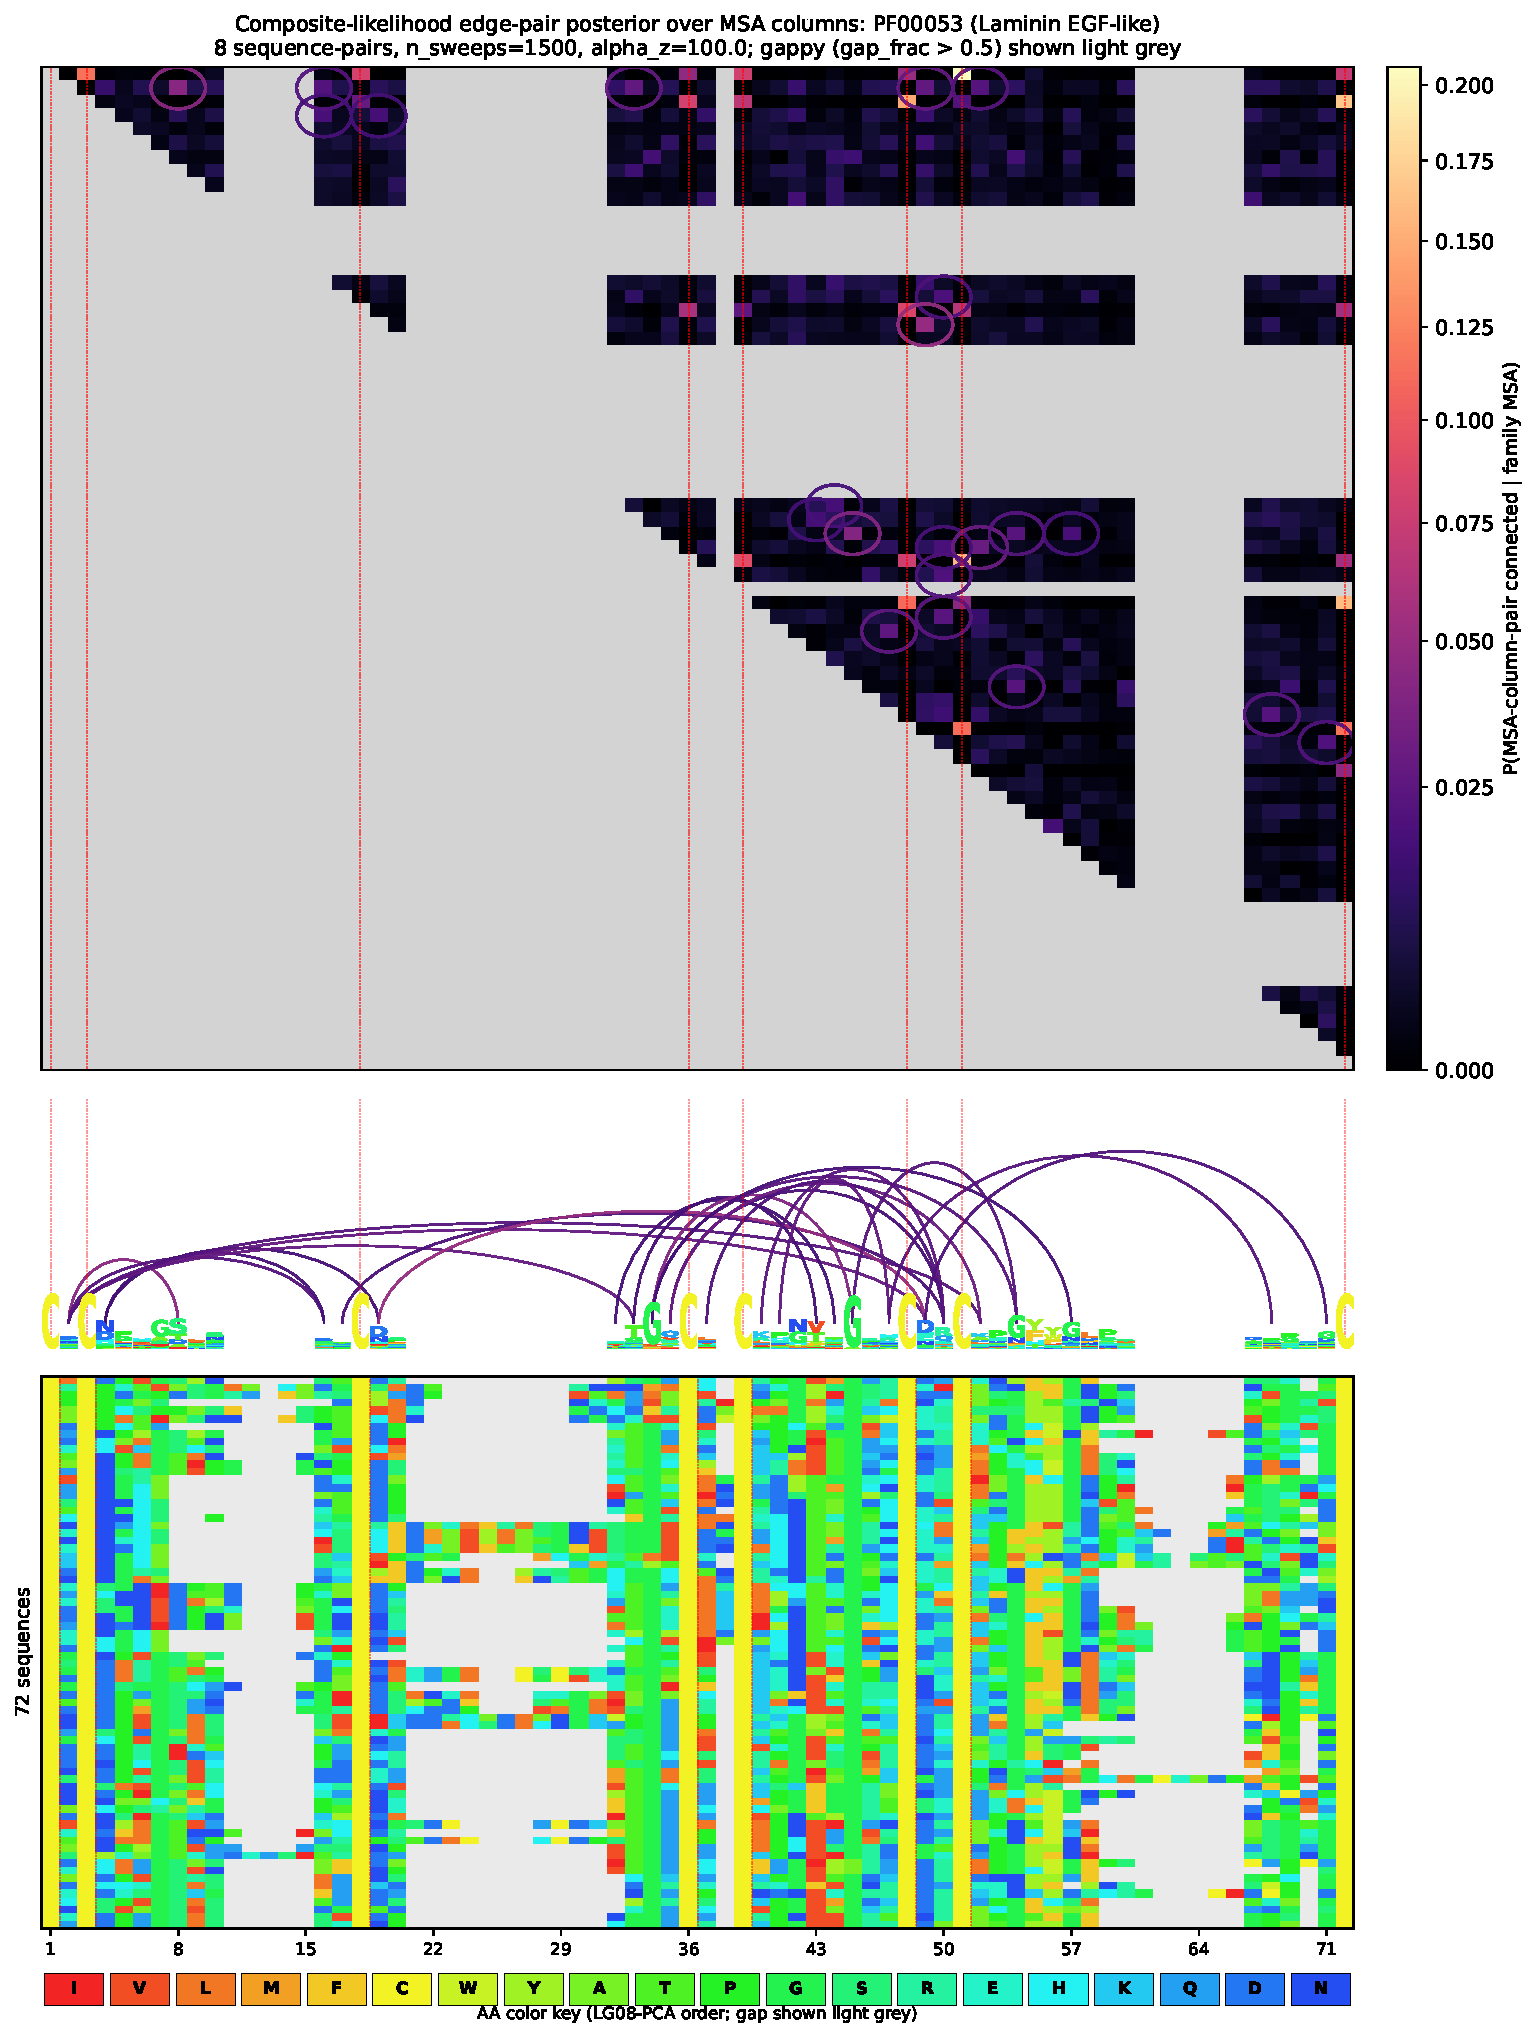
\includegraphics[width=0.8\textwidth]{holmes_msa_triangle_PF00053_K8.pdf}
\caption{\textbf{Composite column-pair posterior across the held-out
\texttt{PF00053} alignment.} \textit{Top:} posterior probability that two
columns of the family MSA share a table, pooled over eight sequence pairs
(columns with more than half gaps in grey). Circles mark the top-ranked
non-cysteine pairs, drawn as arcs over the sequence logo in the middle
panel. \textit{Bottom:} the $72$-sequence MSA, colored by amino acid. All
$28$ candidate Cys--Cys column pairs fall in the top $50$ posteriors.}
\label{fig:pf00053}

{\footnotesize\itshape Alt text: Three stacked panels. The top panel is a
triangular heat map of column-pair posteriors with grey bands for gappy
columns and a few bright cells. The middle panel is a sequence logo with
purple arcs linking pairs of columns. The bottom panel is a colored
multiple alignment of 72 sequences with eight yellow cysteine columns.}
\end{figure}

\subsection{Alignment accuracy on BAliBASE}
\label{sec:balibase}

We scored multiple-alignment accuracy against the BAliBASE~3
\texttt{bali3pdbm} references~\citep{Thompson1999}. The $O(L^4)$ setup of the
pair sampler limits it to sequences shorter than $150$ residues, which leaves
$22$ families and $187$ sequence pairs. For every pair-HMM method the
pairwise posteriors are merged into a multiple alignment by sequence
annealing~\citep{BradleyEtAl2009}, and the result is scored by column $F_1$,
sum-of-pairs (SP) and total-column (TC) scores (\Cref{tab:aln}). For the
\Potts\ rows the posteriors are the running means $Q'$ from the sampler,
with replica exchange over six values of $\alpha_z$ from $100$ to
$5{,}000$, a swap proposed every ten sweeps, $8{,}000$ sweeps after $2{,}000$
of burn-in, and two independent replicates per pair.

\begin{table}[t]
\caption{Multiple-alignment accuracy on BAliBASE~3 \texttt{bali3pdbm},
restricted to families whose sequences are all shorter than $150$ residues
($22$ families, $187$ sequence pairs). Pair-HMM posteriors are merged into
multiple alignments by sequence annealing. TKF92-$K{=}20$ is a mixture of
$20$ TKF92 models. The no-coupling row uses the same eight site classes with
$H=0$. MAFFT~\citep{Katoh2013} and MUSCLE~\citep{Edgar2004} are shown for
reference. All rows are scored on the same $22$ families and $187$ pairs.}
\label{tab:aln}
\centering
\setlength{\tabcolsep}{6pt}
\begin{tabular}{lccc}
\toprule
Method & $F_1$ & SP & TC\\
\midrule
TKF92                                   & 0.514 & 0.724 & 0.631\\
TKF92-$K{=}20$                          & 0.515 & 0.732 & 0.637\\
\Potts, $K_c{=}4$                        & 0.509 & 0.705 & 0.609\\
\Potts, $K_c{=}8$, no coupling           & 0.517 & 0.729 & 0.629\\
\Potts, $K_c{=}8$                        & 0.513 & 0.730 & 0.640\\
\midrule
MAFFT (FFT-NS-2)                        & 0.509 & 0.691 & 0.558\\
MUSCLE (default)                        & 0.512 & 0.760 & 0.662\\
\bottomrule
\end{tabular}
\end{table}

Coupling changes pairwise alignment accuracy only slightly, and not
consistently. The eight-class model is the best of the pair-HMM methods on
TC, $0.009$ above TKF92, and turning its coupling on raises TC by $0.011$ over
the same classes without coupling, while $F_1$ falls by $0.004$. The four-class
model is below TKF92 on all three scores. The pairwise coupling signal is
weak: a single sequence pair gives a boost from only four residues per
candidate pair, and sequence annealing discards the sampled pairings when it
merges the pairwise posteriors. The family-level pooling that sharpens
\Cref{fig:pf00053} is not yet available to the aligner.
%% PROVENANCE (source survey 2026-09-24, verified 2026-09-24):
%%  - TKF92, TKF92-K20, MAFFT, MUSCLE: math-paper/results/balibase_summary_l150.md
%%    (FSA1 columns).  Reproduced exactly.
%%  - Potts K4: ~/tkf-mixdom/python/experiments/expected_balibase/
%%    expected_balibase_inf_phmm_K4_l150_withsps.json; recomputed L<150
%%    aggregate = F1 0.5093 (corpus_hard) / SP 0.7048 / TC 0.6092 over
%%    22 families, 187 pairs.  Cache v11-aws-canonical.
%%  - Potts K8, no-coupling ablation: math-paper/results/
%%    expected_balibase_tkf92_K8_tkfdp.json (120 families); the L<150 subset
%%    recomputes to F1 0.5174 / SP 0.7290 / TC 0.6287 over the same 22
%%    families and 187 pairs.  Written by commit 31da1c9e.
%%  - Potts K8, coupled: run v12-aws-k8-top8000 (checkpoint
%%    K8-KH1-top8000-2026-05-22).  Values recorded in commit 31da1c9e's
%%    message as the "full K=8" comparison (F1 0.5131 / SP 0.7301 /
%%    TC 0.6399); the aggregated JSON was never committed.  Coverage is
%%    confirmed: s3://tkf-mixdom-gpu-<AWS_ACCOUNT>/balibase-runs/
%%    v12-aws-k8-top8000/ holds 187 per-pair Q' results (plus 54 length-
%%    excluded stubs), matching the K4 family/pair split exactly.
%%    Restitch + commit per docs/balibase_187pair_rerun_plan.md (step 0).
%%  - NOT the source for this table: math-paper/results/
%%    downstream_fsa_K8coupled_restricted.json is the same run restricted to
%%    MixFrag's 155-pair coverage for the paper-1 comparison (SP 0.662 /
%%    TC 0.539) and is not comparable to the 187-pair rows above.

% =============================================================
\section{Discussion}
\label{sec:discussion}
% =============================================================

Two substitution processes share one indel skeleton, and each has its
strengths. Energy balancing is faithful to the physics inside a table: it is a
reversible \CTBN, the direct descendant of contact energies, and its sites
respond to one another's current states. Its costs are the Sinkhorn repair,
which grows into a tower of compensatory potentials beyond two guests, its
refusal of simultaneous substitutions, and a likelihood that in principle
depends on unobserved tablemates. Mood lighting is exchangeable and lumpable
by construction, needs one mediator per table at any size, and captures
compensatory swaps directly. Its costs are a fictitious latent field with no
unique physical referent, and the loss of direct dynamical coupling that the
companion paper measures in held-out
likelihood~\citep{LargeHolmes2026Coupled}. At the cap of two guests that we
use for alignment, the choice matters less than it first appears: marginal
consistency reduces to a condition on single-site marginals, and any suitable
two-site chain can be used. Which mechanism is biologically truer, selection
on single moves or shared compensation across a population, is not settled by
the present data.

The unifying requirement is marginal-consistency. It is what reversibility
demands when residues join and leave tables, and it is what keeps the
TKF--DP's alignment prior exactly TKF92's. That in turn licenses the common
practice of conditioning on an alignment and treating gaps as missing data,
while offering an explicit joint model to anyone who wants one. The pairwise
coupling signal is weak, and so are its effects on pairwise alignment
accuracy. The signal is much stronger when pooled over a family, as the
composite posterior on \texttt{PF00053} shows. The obvious next step is a
sampler that shares one partition of columns across all the sequences of a
family, on a tree. The pairwise sampler here is the single-branch marginal of
that object, and the tree version would also carry the augmented histories of
\Cref{sec:consistency} wherever the table process is not lumpable.

Several extensions are natural. The class--archetype map of mood lighting can
carry its own exchangeable prior; restricting it to permutations would narrow
\deF\ toward strictly compensatory swaps. Overlapping clusters would let a
site belong to more than one coupled group, and might suggest an Indian buffet
process~\citep{ibp} in place of the Ewens partition. Finally, two
foundational ideas in this area were energy-based constructions that later
work reframed statistically: the Miyazawa--Jernigan contact
potentials~\citep{Miyazawa1985} that became Potts couplings, and Miyazawa's
alignment partition functions~\citep{Miyazawa1995} that anticipated the
pair HMM Forward likelihood. Going from energy balancing to mood lighting
retraces the same path from energy to statistics.

\label{endofbody}

% =============================================================
\section*{Data availability}
% =============================================================

This study generated no new sequence or structural data. It uses the
\Pfam\ protein families database \citep{Pfam2021} and the BAliBASE~3
reference alignment benchmark \citep{Thompson1999}. Source code for the
models and the sampler, the trained parameters, and the scripts that
regenerate every table and figure in this paper are available at
\url{https://github.com/evoldoers/tkfdp} \citep{TKFDPCode}.

% =============================================================
\section*{Acknowledgements}
% =============================================================

We thank Jeff Thorne, Sean Eddy, Jotun Hein, Debora Marks, Yun Song, Marc
Suchard, Gerton Lunter, Nick Goldman, Nicola De Maio and Elena Rivas for
helpful discussions. Some of the mathematical derivations, exposition and code
in this work were drafted with the assistance of large language models
(Anthropic's Claude and OpenAI's ChatGPT) and were then checked and edited by
the authors, who take full responsibility for the content.

\subsection*{Funding}

This work was supported by the National Institutes of Health
(HG004483, GM080203, HG013117).

% =============================================================
\section*{Conflict of interest}
% =============================================================

The authors declare no conflict of interest.

\newpage
\bibliographystyle{abbrvnat}
\bibliography{refs}

\end{document}
